\chapter{Theory background}
\label{ch:theory}

This chapter presents the technologies that are used in the system developed for this project, putting the emphasis on understanding the main concepts and introducing the terminology and notation required to fully understand the system itself, which is described in the next chapter. This chapter is mostly based on the book \textbf{Dive into Dive Learning (D2L)} \citep{Zhang2019d2l}, published online under a Creative Commons License (CC BY-NC-SA 4.0) with some modifications. In particular, we have excluded the source code, rewritten some paragraphs to keep the consistence with the context in which the material is used, and we have also added material to some parts that were of particular interest for our purposes.

This chapter will cover the following topics:

\begin{itemize}
    \item Convolutional Neural Networks (\cref{sec:cnn})
    \item Recurrent Neural Neworks (\cref{sec:rnn})
    \item Encoder-Decoder Architecture (\cref{sec:encoder-decoder})
    \item Attention Mechanism (\cref{sec:attention})
\end{itemize}

A basic understanding of neural networks is assumed, if not, the reader is referred to some introductory guide. In particular, we recommend chapters 3 and 4 of the D2L book referred above.

\section{Convolutional Neural Networks}\label{sec:cnn}

As we have seen in the encoder-decoder architecture, the encoder used for image captioning is typically a Convolutional Neural Network (CNN). In this section we provide a brief explanation of this kind of network architecture and introduce some of the most remarkable examples, of which some have been used for the system developed in this project.

\subsection{From fully connected layers to convolutions}

2012 was the first year that neural nets grew to prominence as Alex Krizhevsky used them to win that year’s ImageNet Large Scale Visual Recognition Competition (ILSVRC) competition \citep{Krizhevsky2012}, with an astounding drop of the classification error record from 26\% to 15\%. Ever since then, a host of companies have been using deep learning at the core of their services, including Facebook (face recognition), Google (photo search, translation, voice recognition), Amazon (product recommendations), Pinterest (feed personalization), and Instagram (search infrastructure), amongst others.

Classical neural networks, as the Multi-Layer Perceptron (MLP), and fully connected architectures in general, were designed to work with tabular data, that is, data consisting of rows corresponding to examples and columns corresponding to features. With tabular data, we might anticipate that pattern we seek could require modeling interactions among the features, but do not assume anything a priori about which features are related to each other or in what way. In such cases, there is no way of exploiting such interactions when designing the network architecture, and MLPs are probably the best approach. However, once we start dealing with high-dimensional perceptual data, these "structure-less" networks can grow very unwieldy. 

For instance, let’s consider the task of classifying pictures into either cats or dogs. Say that we do a thorough job in data collection, collecting an annotated set of high-quality 1-megapixel photographs. This means that the input into a network has 1 million dimensions. Even an aggressive reduction to 1,000 hidden dimensions would require a dense (fully-connected) layer to support  $10^9$  parameters. Unless we have an extremely large dataset (perhaps billions?), lots of GPUs, a talent for extreme distributed optimization, and an extraordinary amount of patience, learning the parameters of this network may turn out to be impossible.

A careful reader might object to this argument on the basis that 1 megapixel resolution may not be necessary. However, while you could get away with 100,000 pixels, we grossly underestimated the number of hidden nodes that it typically takes to learn good hidden representations of images. Learning a binary classifier with so many parameters might seem to require that we collect an enormous dataset, perhaps comparable to the number of dogs and cats on the planet. And yet both humans and computers are able to distinguish cats from dogs quite well, seemingly contradicting these conclusions. That’s because images exhibit rich structure that is typically exploited by humans and machine learning models alike. For example, when perceiving images, the are two important properties that our visual systems use:

\begin{itemize}
    \item \textit{Translation invariance}: vision should respond similarly to the same object regardless of where it appears in the image.
    \item \textit{Locality}: for certain tasks our vision should focus on local regions, without regard for what else is happening in the image at greater distances.
\end{itemize}

Convolutional Neural Networks, or \textit{ConvNets}, for short, are a kind of artificial neural networks designed specifically to benefit  from these properties of the visual system. Whilst fully connected (dense) layers. 

ConvNets were inspired by biological processes in that the connectivity pattern between neurons resembles the organization of the animal visual cortex. Individual cortical neurons respond to stimuli only in a restricted region of the visual field known as the receptive field. The receptive fields of different neurons partially overlap such that they cover the entire visual field.

ConvNets get their name from a mathematical operation called \textbf{convolution}, although they actually correspond to a very similar operation called \textit{cross-correlation}, represented by an asterisk within a circle, $\circledast$. 

ConvNets are built by chaining multiple layers of units that apply two types of operation: convolutions and pooling. Let's briefly review how these operations work in practice:

\subsection{Convolution layers}\label{subsec:conv_layers}

\subsubsection{The Cross-correlation operation}

The most important operation performed by ConvNets is the cross-correlation operation (often called \textit{convolution} operation), which take an input array and a \textbf{correlation kernel} array, and produce an output array through a \textbf{cross-correlation operation}. Images are represented as 2D arrays of pixels, plus a third dimension when color channels are considered. But for the sake of simplicity, let's start with a 2D representation of images. 

\begin{figure}[hpt]
	\centering
	\includesvg{images/ch3/correlation.svg}
	\caption{Two dimensional cross-correlation operation. The shaded portions are the first output element and the input and kernel array elements used in its computation: $0 \times 0+1 \times 1+3 \times 2+4 \times 3=19$}
	\label{fig:correlation}
\end{figure}

In the two-dimensional cross-correlation operation (\cref{fig:correlation}), we begin with the convolution window positioned at the top-left corner of the input array and slide it across the input array, both from left to right and top to bottom. When the convolution window slides to a certain position, the input subarray contained in that window and the kernel array are multiplied (element-wise) and the resulting array is summed up yielding a single scalar value. This result is precisely the value of the output array at the corresponding location. Here, the output array has a height of 2 and width of 2 and the four elements are derived from the two-dimensional cross-correlation operation:

\begin{align*}
0 \times 0+1 \times 1+3 \times 2+4 \times 3=19,\\
1 \times 0+2 \times 1+4 \times 2+5 \times 3=25,\\
3 \times 0+4 \times 1+6 \times 2+7 \times 3=37,\\
4 \times 0+5 \times 1+7 \times 2+8 \times 3=43.
\end{align*}

Note that along each axis, the output array is slightly smaller than the input. Because the kernel has a width greater than one, and we can only computer the cross-correlation for locations where the kernel fits wholly within the image, the output size is given by the input size $H \times W$  minus the size of the convolutional kernel $h \times w$ via $(H-h+1)\times(W-w+1)$. This is the case since we need enough space to ‘shift’ the convolutional kernel across the image.

A convolutional layer cross-correlates the input and kernels and adds a scalar bias $b$ to produce an output. The parameters of the convolutional layer are precisely the values that constitute the kernel and the scalar bias. When training the models based on convolutional layers, we typically initialize the kernels randomly, just as we would with a fully-connected layer. 

%Optionally, a convolutional layer may also apply an activation function $g$ to produce its final output, so we can define the output of a convolutional layer as:
%$$Y_i = g(b_j + \sum_i{K_{ij}\circledast Y_i}$$

\textit{Correlation kernels}, often called \textit{convolution filters}, can be seen as feature detectors; for example, they can be used to detect edges in different orientations, such as vertical lines, horizontal lines, or curves of any shape. Designing an edge detector by finite differences $[1, -1]$ is neat if we know this is precisely what we are looking for. However, as we look at larger kernels, and consider successive layers of convolutions, it might be impossible to specify precisely what each filter should be doing manually. Fortunately, we do not need to define kernels by hand, since they can be learned automatically using backpropagation, as the weights of a fully connected layer.

\begin{figure}[hpt]
	\centering
	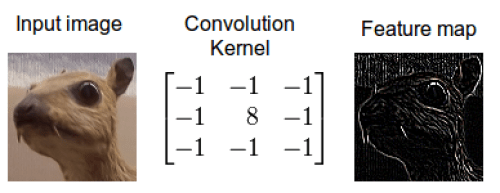
\includegraphics[scale=0.7]{images/ch3/edge-detection.png}
	\caption{Example of a convolution kernel for edge detection}
	\label{fig:edge-detection}
\end{figure}

\subsubsection{Padding}

In the previous example, our input had a height and width of 3 and a convolution kernel with a height and width of 2, yielding an output with a height and a width of 2. In general, assuming the input shape is  $n_h \times n_w$  and the convolution kernel window shape is $k_h \times k_w$, then the output shape will be

$$(n_h-k_h+1) \times (n_w-k_w+1)$$
 
Therefore, the output shape of the convolutional layer is determined by the shape of the input and the shape of the convolution kernel window.

In several cases we might want to incorporate particular techniques --padding and strides-- regarding the size of the output:
\begin{itemize}
    \item In general, since kernels generally have width and height greater than 1, that means that after applying many successive convolutions, we will wind up with an output that is much smaller than our input. If we start with a $240\times240$ pixel image, 10 layers of $5\times5$ convolutions reduce the image to $200\times200$ pixels, slicing off 30\% of the image and with it obliterating any interesting information on the boundaries of the original image. Padding handles this issue.
    \item In some cases, we want to reduce the resolution drastically if say we find our original input resolution to be unwieldy. Strides can help in these instances.
\end{itemize}

\begin{figure}[hpt]
	\centering
	\includesvg{images/ch3/conv_pad.svg}
	\caption{Two-dimensional cross-correlation with padding. The shaded portions are the input and kernel array elements used by the first output element: $0\times0+0\times1+0\times2+0\times3=0$}
	\label{fig:conv_pad}
\end{figure}

In general, if we add a total of  $p_h$  rows of padding (roughly half on top and half on bottom) and a total of  $p_w$  columns of padding (roughly half on the left and half on the right), the output shape will be

$$(n_h-k_h+p_h+1)\times(n_w-k_w+p_w+1)$$
 
This means that the height and width of the output will increase by  $p_h$  and  $p_w$  respectively.

In many cases, we will want to set  $p_h=k_h-1$  and  $p_w=k_w-1$  to give the input and output the same height and width. This will make it easier to predict the output shape of each layer when constructing the network. Assuming that  $k_h$  is odd here, we will pad  $p_h/2$ rows on both sides of the height. If $k_h$  is even, one possibility is to pad  $\lceil p_h/2\rceil$  rows on the top of the input and  $\lfloor p_h/2\rfloor$  rows on the bottom. We will pad both sides of the width in the same way.

ConvNets commonly use correlation kernels with odd height and width values, such as 1, 3, 5, or 7. Choosing odd kernel sizes has the benefit that we can preserve the spatial dimensionality while padding with the same number of rows on top and bottom, and the same number of columns on left and right.

Moreover, this practice of using odd kernels and padding to precisely preserve dimensionality offers a clerical benefit. For any two-dimensional array $X$, when the kernels size is odd and the number of padding rows and columns on all sides are the same, producing an output with the same height and width as the input, we know that the output $Y[i,j]$ is calculated by cross-correlation of the input and convolution kernel with the window centered on $X[i,j]$.

In the following example, we create a two-dimensional convolutional layer with a height and width of 3 and apply 1 pixel of padding on all sides. Given an input with a height and width of 8, we find that the height and width of the output is also 8.

\subsubsection{Stride}

When computing the cross-correlation, we start with the convolution window at the top-left corner of the input array, and then slide it over all locations both down and to the right. In previous examples, we default to sliding one pixel at a time. However, sometimes, either for computational efficiency or because we wish to downsample, we move our window more than one pixel at a time, skipping the intermediate locations.

We refer to the number of rows and columns traversed per slide as the stride. So far, we have used strides of 1, both for height and width. Sometimes, we may want to use a larger stride. The figure below shows a two-dimensional cross-correlation operation with a stride of 3 vertically and 2 horizontally. We can see that when the second element of the first column is output, the convolution window slides down three rows. The convolution window slides two columns to the right when the second element of the first row is output. When the convolution window slides two columns to the right on the input, there is no output because the input element cannot fill the window (unless we add padding).

\begin{figure}[hpt]
	\centering
	\includesvg{images/ch3/conv_stride.svg}
	\caption{Cross-correlation with strides of 3 and 2 for height and width respectively. The shaded portions are the output element and the input and core array elements used in its computation: $0\times0+0\times1+1\times2+2\times3=8,  0\times0+6\times1+0\times2+0\times3=6$}
	\label{fig:conv_stride}
\end{figure}

In general, when the stride for the height is $s_h4  and the stride for the width is s_w$ , the output shape is

$$\lfloor(n_h-k_h+p_h+s_h)/s_h\rfloor \times \lfloor(n_w-k_w+p_w+s_w)/s_w\rfloor$$
 
If we set $p_h=k_h-1$  and  $p_w=k_w-1$ , then the output shape will be simplified to $\lfloor(n_h+s_h-1)/s_h\rfloor \times \lfloor(n_w+s_w-1)/s_w\rfloor$. Going a step further, if the input height and width are divisible by the strides on the height and width, then the output shape will be $(n_h/s_h)\times(n_w/s_w)$.

For the sake of brevity, when the padding number on both sides of the input height and width are $p_h$  and $p_w$  respectively, we call the padding $(p_h,p_w)$. Specifically, when  $p_h=p_w=p$, the padding is $p$. When the strides on the height and width are $s_h$ and $s_w$, respectively, we call the stride $(s_h,s_w)$. Specifically, when $s_h=s_w=s$, the stride is $s$. By default, the padding is 0 and the stride is 1. In practice we rarely use inhomogeneous strides or padding, i.e., we usually have $p_h=p_w$ and $s_h=s_w$.

\subsubsection{Multiple Input and Output Channels}

While we have described the multiple channels that comprise each image (e.g. color images have the standard RGB channels to indicate the amount of red, green and blue), until now, we simplified all of our numerical examples by working with just a single input and a single output channel. This has allowed us to think of our inputs, convolutional kernels, and outputs each as two-dimensional arrays.

When we add channels into the mix, our inputs and hidden representations both become three-dimensional arrays. For example, each RGB input image has shape $3\times h\times w$. We refer to this axis, with a size of 3, as the channel dimension. In this section, we will take a deeper look at convolution kernels with multiple input and multiple output channels.

\paragraph{Multiple Input Channels}

When the input data contains multiple channels, we need to construct a convolution kernel with the same number of input channels as the input data, so that it can perform cross-correlation with the input data. Assuming that the number of channels for the input data is $c_i$, the number of input channels of the convolution kernel also needs to be $c_i$. If our convolution kernel’s window shape is $k_h\times k_w$, then when $c_i=1$, we can think of our convolution kernel as just a two-dimensional array of shape $k_h\times k_w$.

However, when $c_i>1$, we need a kernel that contains an array of shape $k_h\times k_w$ for each input channel. Concatenating these $c_i$ arrays together yields a convolution kernel of shape $c_i\times k_h\times k_w$. Since the input and convolution kernel each have $c_i$ channels, we can perform a cross-correlation operation on the two-dimensional array of the input and the two-dimensional kernel array of the convolution kernel for each channel, adding the $c_i$ results together (summing over the channels) to yield a two-dimensional array. This is the result of a two-dimensional cross-correlation between multi-channel input data and a multi-input channel convolution kernel.

In the figure below, we demonstrate an example of a two-dimensional cross-correlation with two input channels. The shaded portions are the first output element as well as the input and kernel array elements used in its computation:

$$(1 \times 1+2\times2+4\times3+5\times4)+(0\times0+1 \times 1+3\times2+4\times3)=56$$

\begin{figure}[hpt]
	\centering
	\includesvg{images/ch3/conv_multi_in.svg}
	\caption{Cross-correlation computation with 2 input channels. The shaded portions are the first output element as well as the input and kernel array elements used in its computation:  $(1 \times 1+2 \times 2+4\times3+5\times4)+(0\times0+1 \times 1+3\times2+4\times3)=56.$}
	\label{fig:conv_multi_in}
\end{figure}

\paragraph{Multiple Output Channels}

Regardless of the number of input channels, so far we always ended up with one output channel. However, as we discussed earlier, it turns out to be essential to have multiple channels at each layer. In the most popular neural network architectures, we actually increase the channel dimension as we go higher up in the neural network, typically downsampling to trade off spatial resolution for greater channel depth. Intuitively, you could think of each channel as responding to some different set of features. Reality is a bit more complicated than the most naive intepretations of this intuition since representations are not learned independently but are rather optimized to be jointly useful. So it may not be that a single channel learns an edge detector but rather that some direction in channel space corresponds to detecting edges.

Denote by $c_i$ and $c_o$  the number of input and output channels, respectively, and let $k_h$ and $k_w$ be the height and width of the kernel. To get an output with multiple channels, we can create a kernel array of shape $c_i \times k_h \times k_w$ for each output channel. We concatenate them on the output channel dimension, so that the shape of the convolution kernel is $c_o \times c_i \times k_h \times k_w$. In cross-correlation operations, the result on each output channel is calculated from the convolution kernel corresponding to that output channel and takes input from all channels in the input array.

\paragraph{$1 \times 1$ convolutional layers}

At first, a $1 \times 1$  convolution, i.e.  $k_h=k_w=1$, does not seem to make much sense. After all, a convolution correlates adjacent pixels. A $1 \times 1$ convolution obviously does not. Nonetheless, they are popular operations that are sometimes included in the designs of complex deep networks. Let’s see in some detail what it actually does.

Because the minimum window is used, the $1 \times 1$ convolution loses the ability of larger convolutional layers to recognize patterns consisting of interactions among adjacent elements in the height and width dimensions. The only computation of the $1 \times 1$ convolution occurs on the channel dimension.

\cref{fig:conv_1x1} shows the cross-correlation computation using the $1 \times 1$ convolution kernel with 3 input channels and 2 output channels. Note that the inputs and outputs have the same height and width. Each element in the output is derived from a linear combination of elements at the same position in the input image. You could think of the $1 \times 1$  convolutional layer as constituting a fully-connected layer applied at every single pixel location to transform the $c_i$ corresponding input values into $c_o$ output values. Because this is still a convolutional layer, the weights are tied across pixel location Thus the $1 \times 1$  convolutional layer requires $c_o \times c_i$ weights (plus the bias terms).

\begin{figure}[hpt]
	\centering
	\includesvg{images/ch3/conv_1x1.svg}
	\caption{Cross-correlation computation using a $1 \times 1$ convolution kernel with 3 input channels and 2 output channels. The inputs and outputs have the same height and width.}
	\label{fig:conv_1x1}
\end{figure}

\subsection{Pooling layers}\label{subsec:pool_layers}

Often, as we process images, we want to gradually reduce the spatial resolution of our hidden representations, aggregating information so that the higher up we go in the network, the larger the receptive field (in the input) to which each hidden node is sensitive.

Often our ultimate task asks some global question about the image, e.g., does it contain a cat? So typically the nodes of our final layer should be sensitive to the entire input. By gradually aggregating information, yielding coarser and coarser maps, we accomplish this goal of ultimately learning a global representation, while keeping all of the advantages of convolutional layers at the intermediate layers of processing.

Moreover, when detecting lower-level features, such as edges, we often want our representations to be somewhat invariant to translation. For instance, if we take the image X with a sharp delineation between black and white and shift the whole image by one pixel to the right, i.e. $Z[i,j] = X[i,j+1]$ then the output for for the new image Z might be vastly different. The edge will have shifted by one pixel and with it all the activations. In reality, objects hardly ever occur exactly at the same place. In fact, even with a tripod and a stationary object, vibration of the camera due to the movement of the shutter might shift everything by a pixel or so.

Pooling layers serve the dual purposes of mitigating the sensitivity of convolutional layers to location and of spatially downsampling representations.

\subsubsection{Maximum Pooling and Average Pooling}

Like convolutional layers, pooling layers apply a fixed-shape window that slides over all regions in the input according to its stride, computing a single output for each location traversed by the fixed-shape window (sometimes known as the pooling window). However, unlike convolutional layers, which need parameters to represent the correlation kernels, the pooling layer contains no parameters (there is no kernel). Instead, pooling operators are deterministic, typically calculating either the maximum or the average value of the elements in the pooling window. These operations are called maximum pooling (\textit{max pooling} for short) and \textit{average pooling}, respectively.

In both cases, as with the cross-correlation operator, we can think of the pooling window as starting from the top left of the input array and sliding across the input array from left to right and top to bottom. At each location that the pooling window hits, it computes the maximum or average value of the input subarray in the window (depending on whether max or average pooling is employed).

\begin{figure}[hpt]
	\centering
	\includesvg{images/ch3/pooling.svg}
	\caption{Maximum pooling with a pooling window shape of $2\times2$. The shaded portions represent the first output element and the input element used for its computation:  $\max(0,1,3,4)=4$.}
	\label{fig:pooling}
\end{figure}

The output array in \cref{fig:pooling} has a height of 2 and a width of 2. The four elements are derived from the maximum value of $\text{max}$:

\begin{align*}
\max(0,1,3,4)=4,\\
\max(1,2,4,5)=5,\\
\max(3,4,6,7)=7,\\
\max(4,5,7,8)=8.\\
\end{align*}

A pooling layer with a pooling window shape of $p \times q$ is called a $p \times q$ pooling layer. The pooling operation is called $p \times q$ pooling.

Let us return to the object edge detection example mentioned at the beginning of this section. Now we will use the output of the convolutional layer as the input for $2 \times 2$  max pooling. Set the convolutional layer input as $X$ and the pooling layer output as $Y$. Whether or not the values of $X[i, j]$ and $X[i, j+1]$ are different, or $X[i, j+1]$ and $X[i, j+2]$ are different, the pooling layer outputs all include $Y[i, j]=1$. That is to say, using the $2 \times 2$ maximum pooling layer, we can still detect if the pattern recognized by the convolutional layer moves no more than one element in height and width.

\subsubsection{Padding and Stride}

As with convolutional layers, pooling layers can also change the output shape. And as before, we can alter the operation to achieve a desired output shape by padding the input and adjusting the stride.

When processing multi-channel input data, the pooling layer pools each input channel separately, rather than adding the inputs of each channel by channel as in a convolutional layer. This means that the number of output channels for the pooling layer is the same as the number of input channels

% \subsection{Summary of ConvNets}

% \begin{itemize}
%     \item Translation invariance in images implies that all patches of an image will be treated in the same manner.
%     \item Locality means that only a small neighborhood of pixels will be used for computation.    
%     \item Channels on input and output allows for meaningful feature analysis.
%     \item The core computation of a two-dimensional convolutional layer is a two-dimensional cross-correlation operation. In its simplest form, this performs a cross-correlation operation on the two-dimensional input data and the kernel, and then adds a bias.
%     \item We can design a kernel to detect edges in images.
%     \item We can learn the kernel through data
%     \item Padding can increase the height and width of the output. This is often used to give the output the same height and width as the input.
%     \item The stride can reduce the resolution of the output, for example reducing the height and width of the output to only  $1/n$  of the height and width of the input ($n$  is an integer greater than 1)
%     \item Padding and stride can be used to adjust the dimensionality of the data effectively.
%     \item Multiple channels can be used to extend the model parameters of the convolutional layer.
%     \item The $1 \times 1$ convolutional layer is equivalent to the fully-connected layer, when applied on a per pixel basis.
%     \item The $1 \times 1$  convolutional layer is typically used to adjust the number of channels between network layers and to control model complexity.
%     \item Taking the input elements in the pooling window, the maximum pooling operation assigns the maximum value as the output and the average pooling operation assigns the average value as the output.
%     \item One of the major functions of a pooling layer is to alleviate the excessive sensitivity of the convolutional layer to location.
%     \item We can specify the padding and stride for the pooling layer.
%     \item Maximum pooling, combined with a stride larger than 1 can be used to reduce the resolution.
%     \item The pooling layer’s number of output channels is the same as the number of input channels.
% \end{itemize}

\subsection{Examples of concrete CNN architectures}

\subsubsection{Classical convolutional networks: LeNet}

In this section, we will introduce one of the first published convolutional neural networks whose benefit was first demonstrated by  \citet{Lecun1998}, for the purpose of recognizing handwritten digits in images. In the 90s, their experiments with \href{LeNet}{http://yann.lecun.com/exdb/lenet/} gave the first compelling evidence that it was possible to train convolutional neural networks by backpropagation. Their model achieved outstanding results at the time (only matched by Support Vector Machines at the time) and was adopted to recognize digits for processing deposits in ATM machines. Some ATMs still runn the code that Yann and his colleague Leon Bottou wrote in the 1990s.

In a rough sense, we can think LeNet as consisting of two parts: (i) a block of convolutional layers; and (ii) a block of fully-connected layers. Before getting into the weeds, let’s briefly review the model in \cref{fig:letnet}

\begin{figure}[hpt]
	\centering
	\includesvg[scale=0.4]{images/ch3/lenet.svg}
	\caption{Data flow in LeNet 5. The input is a handwritten digit, the output a probabilitiy over 10 possible outcomes.}
	\label{fig:lenet}
\end{figure}

The basic units in the convolutional block are a convolutional layer and a subsequent average pooling layer (note that max-pooling works better, but it had not been invented in the 90s yet). The convolutional layer is used to recognize the spatial patterns in the image, such as lines and the parts of objects, and the subsequent average pooling layer is used to reduce the dimensionality. The convolutional layer block is composed of repeated stacks of these two basic units. Each convolutional layer uses a $5 \times 5$  kernel and processes each output with a \textit{sigmoid} activation function (again, note that \textit{ReLU}s are now known to work more reliably, but had not been invented yet). The first convolutional layer has 6 output channels, and second convolutional layer increases channel depth further to 16.

However, coinciding with this increase in the number of channels, the height and width are shrunk considerably. Therefore, increasing the number of output channels makes the parameter sizes of the two convolutional layers similar. The two average pooling layers are of size  $2 \times 2$  and take stride 2 (note that this means they are non-overlapping). In other words, the pooling layer downsamples the representation to be precisely one quarter the pre-pooling size.

The convolutional block emits an output with size given by (batch size, channel, height, width). Before we can pass the convolutional block’s output to the fully-connected block, we must flatten each example in the mini-batch. In other words, we take this 4D input and transform it into the 2D input expected by fully-connected layers: as a reminder, the first dimension indexes the examples in the mini-batch and the second gives the flat vector representation of each example. LeNet’s fully-connected layer block has three fully-connected layers, with 120, 84, and 10 outputs, respectively. Because we are still performing classification, the 10 dimensional output layer corresponds to the number of possible output classes.

Summing up: 
\begin{itemize}
    \item A convolutional neural network (in short, ConvNet) is a network using convolutional layers.
    \item In a ConvNet we alternate between convolutions, nonlinearities and often also pooling operations.
    \item Ultimately the resolution is reduced prior to emitting an output via one (or more) dense layers.
    \item LeNet was the first successful deployment of such a network.
\end{itemize}

\subsubsection{Modern architectures}

Although convolutional neural networks were well known in the computer vision and machine learning communities following the introduction of LeNet, they did not immediately dominate the field. Although LeNet achieved good results on early small data sets, the performance and feasibility of training convolutional networks on larger, more realistic datasets had yet to be established
In fact, for much of the intervening time between the early 1990s and the watershed results of 2012, neural networks were often surpassed by other machine learning methods, such as support vector machines.

A major breakthrough came when Alex Krizhevsky and Ilya Sutskever implemented a deep convolutional neural network that could run on GPU hardware. They realized that the computational bottlenecks in CNNs (convolutions and matrix multiplications) are all operations that could be parallelized in hardware. Using two NIVIDA GTX 580s with 3GB of memory, they implemented fast convolutions. The code \href{https://code.google.com/archive/p/cuda-convnet/}{cuda-convnet} was good enough that for several years it was the industry standard and powered the first couple years of the deep learning boom.

\paragraph{AlexNet: first large-scale convnet, beating classical methods in computer vision}


AlexNet was introduced in 2012, named after Alex Krizhevsky, the first author of the breakthrough ImageNet classification paper \citep{Krizhevsky2012}. AlexNet, which employed an 8-layer convolutional neural network, won the ImageNet Large Scale Visual Recognition Challenge 2012 by a phenomenally large margin. This network proved, for the first time, that the features obtained by learning can transcend manually-design features, breaking the previous paradigm in computer vision. The architectures of AlexNet and LeNet are \textit{very similar}, as the diagram below illustrates. Note that we provide a slightly streamlined version of AlexNet removing some of the design quirks that were needed in 2012 to make the model fit on two small GPUs.

\begin{figure}[hpt]
	\centering
	\includesvg[scale=0.8]{images/ch3/alexnet-all.svg}
	\caption{LeNet (left) and AlexNet (right)}
	\label{fig:alexnet}
\end{figure}

The design philosophies of AlexNet and LeNet are very similar, but there are also significant differences. First, AlexNet is much deeper than the comparatively small LeNet5. AlexNet consists of eight layers: five convolutional layers, two fully-connected hidden layers, and one fully-connected output layer. Second, AlexNet used the ReLU instead of the sigmoid as its activation function.

\paragraph{VGG: network architecture based on repeating blocks}

While AlexNet proved that deep convolutional neural networks can achieve good results, it didn't offer a general template to guide subsequent researchers in designing new networks.  In the following sections, we will introduce several heuristic concepts commonly used to design deep networks.

Progress in this field mirrors that in chip design where engineers went from placing transistors to logical elements to logic blocks. Similarly, the design of neural network architectures  had grown progressively more abstract, with researchers moving from thinking in terms of individual neurons to whole layers, and now to blocks, repeating patterns of layers.

The idea of using blocks first emerged from the \href{http://www.robots.ox.ac.uk/~vgg/}{Visual Geometry Group} (VGG) at Oxford University. In their eponymously-named VGG network, It's easy to implement these repeated structures in code with any modern deep learning framework by using loops and subroutines. 

The basic building block of classic convolutional networks is a sequence of the following layers: (i) a convolutional layer  (with padding to maintain the resolution), (ii) a nonlinearity such as a ReLu.

One VGG block consists of a sequence of convolutional layers,  followed by a max pooling layer for spatial downsampling. In the original VGG paper \citet{Simonyan2015} employed convolutions with $3\times3$ kernels and $2 \times 2$ max pooling with stride of $2$ (halving the resolution after each block).

Like AlexNet and LeNet, the VGG Network can be partitioned into two parts: the first consisting mostly of convolutional and pooling layers and a second consisting of fully-connected layers. The convolutional portion of the net connects several \textit{vgg block} modules in succession.

\begin{figure}[hpt]
	\centering
	\includesvg[scale=0.8]{images/ch3/vgg.svg}
	\caption{Designing a network from building blocks}
	\label{fig:vgg}
\end{figure}

The original VGG network had 5 convolutional blocks, among which the first two have one convolutional layer each and the latter three contain two convolutional layers each. The first block has 64 output channels and each subsequent block doubles the number of output channels, until that number reaches $512$. Since this network uses $8$ convolutional layers and $3$ fully-connected layers, it is often called VGG-11.

\paragraph{GoogleLeNet (aka Inception): using parallel concatenations}

\paragraph{ResNet: residual networks}

\paragraph{DenseNet: densely connected architecture}

